\documentclass[../main.tex]{subfiles}

\begin{document}
This chapter is a detailed look at how the outlier detector is actually implemented. We
put special emphasis on the mathematical considerations behind each step and how they
reflect on the actual code. The whole library is freely available at \url{https://github.com/arnaumas/mknn_homology/}. 

\section{Why mutual \texorpdfstring{\( k \)}{k}-nearest neighbours graphs?}
As stated in \cref{sec:prior work}, the first approach to identify clusters and outliers
in a dataset was by finding the maximal cliques of the mutual \( k \)-nearest neighbours
graph, \MKNN graph for short. Let's describe how it is constructed to understand why it is
useful. 

One starts with the nearest neighbours graph. Given a point cloud, \( C
\), its Nearest Neighbour directed graph is constructed according to the following
prescription: there is an edge from \( p \) to \( q \) if and only if \( d(p,q) = \min_{r
	\in C} d(p,r) \), so \( q \) is the closest point to \( p \), its \emph{nearest
neighbour}. The reason the graph is directed is because the relation of being a nearest
neighbour is not symmetric. Indeed, consider three points \( p_1, p_2, p_3 \) which all
lie in a straight line in this order. Let \( d_{12} = d(p_1, p_2) \)  and \( d_{23} =
d(p_2,p_3) \) and suppose \( d_{12} < d_{23} \). Then, \( p_2 \) is \( p_1 \)'s
nearest-neighbour, and vice versa. Yet \( p_2 \) is also \( p_3 \)'s nearest neighbour but
neither \( p_1 \) nor \( p_2 \) are a nearest neighbour of \( p_3 \).

This generalises to the \( k \)-nearest neighbours graph, in which each point is connected
to its \( k \)-th nearest neighbours, that is, the \( k \)-th closest points to it. The
resulting graph is still directed. We obtain the undirected \emph{mutual} \( k \)-nearest
neighbours graph by connecting two points if and only if there are edges between them
in both directions, i.e. if they are \emph{mutual} \( k \)-nearest neighbours. 

\begin{figure}[htb]
	\centering
	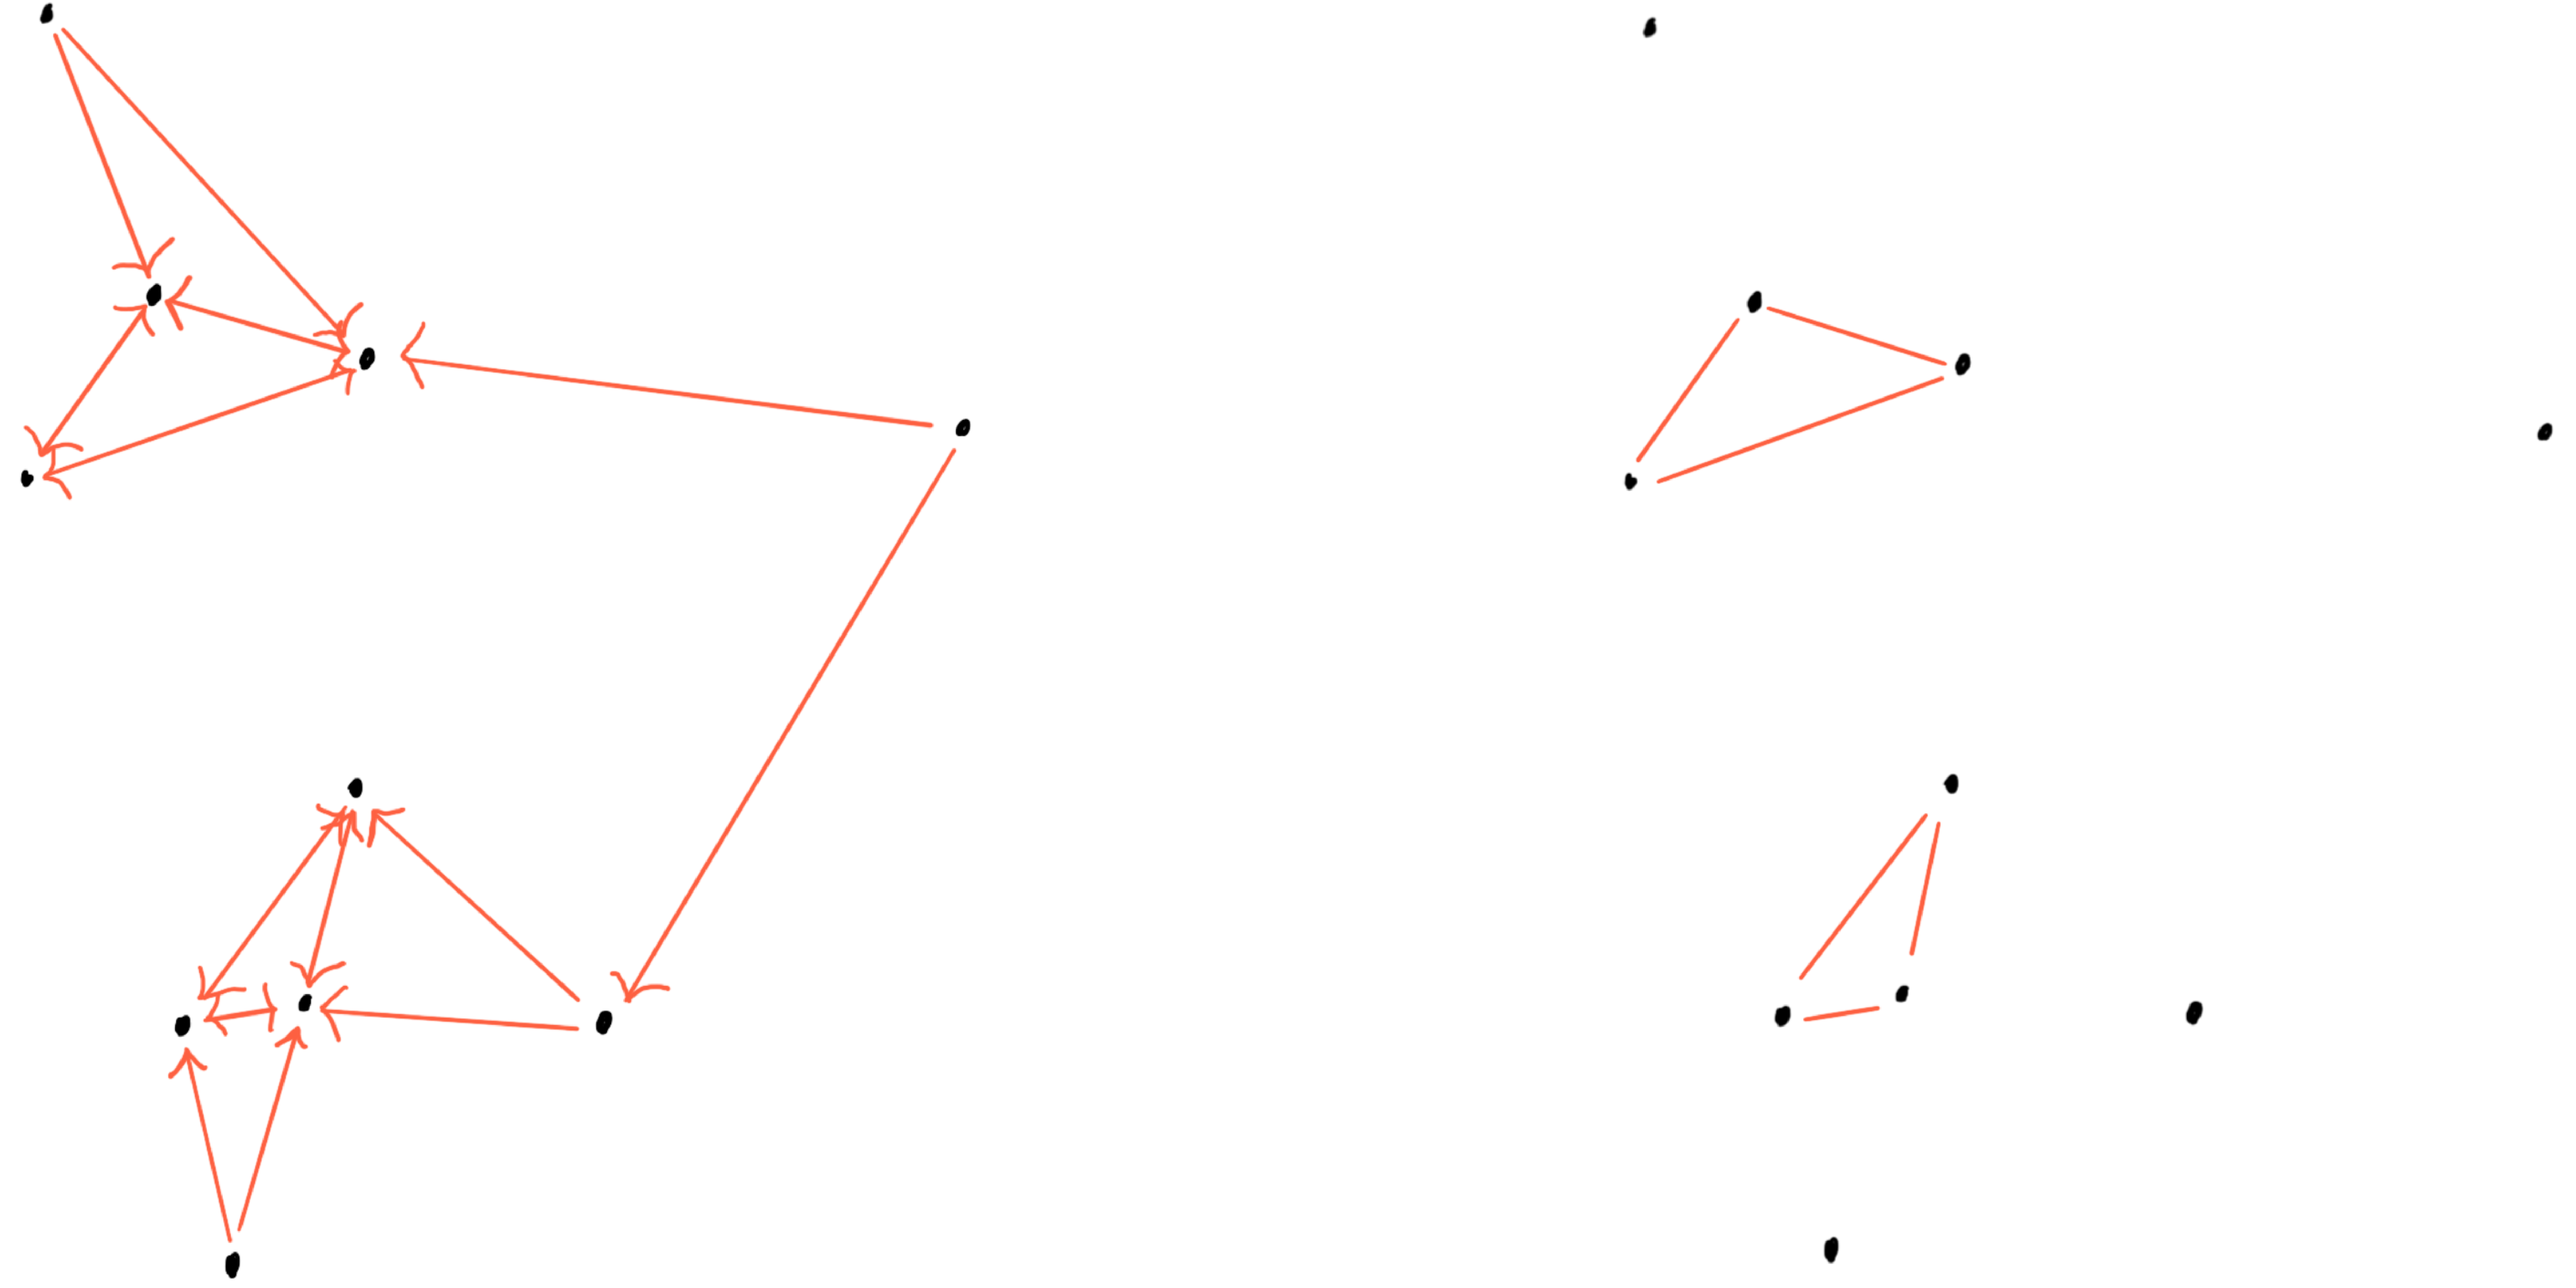
\includegraphics[width = 15cm]{drawings/mknn}
	\caption{The 2NN and M2NN graphs for the same dataset. Note how the M2NN graph is
	undirected and has a lot less edges.}
	\label{fig:mknn}
\end{figure}

Looking at \cref{fig:mknn} we see the 2-nearest neighbours and mutual 2-nearest neighbours
graphs for the same point cloud. In a \( k \)NN	 graph, it is always the case that every
vertex has \( k \) edges, which means that even points which are far away from any cluster
are connected to some other points. This is not very useful if we wish to detect outliers.
However, when taking the \emph{mutual} version, many of this edges disappear. Indeed, now,
for an outlier to become connected to a cluster a higher \( k \) will be required so that
every point within the cluster has become connected to all of its immediate neighbours and
is forced to ``look'' outside the cluster for additional neighbours. This idea of waiting
for a higher \( k \) is exactly the one we exploit when combining the \MKNN graph with
persistent homology, for outliers will presumably become classes in	\( H_0 \) with few
elements and with a long lifetime. 

\section{The steps of the detector}
The whole process from input to output is roughly divided in four steps. First, the data is
shaped into an expected format and wrapped in a class which knows how to compute its
\MKNN	graph for any \( k \). Then, the filtration is built and suitably stored. Finally
the actual computation of the persistence homology takes place. And then, based on the
results of the persistent homology, each point is given an ``outlier-ness'' score. 

\subsection{Constructing the M\texorpdfstring{\( k \)}{k}NN graph}
The input is assumed to be in the form of a \textsf{NumPy} array of shape \( (N,d) \)
where \( N \) is the number of points and \( d \) the number of features or equivalently
the ambient dimension. This array is wrapped in an instance of the class \texttt{Cloud}
which implements a method to compute the \MKNN graph for a given \( k \). 

The procedure to encode this graph is as follows. First, the distance matrix, \( D \), for
the data set is computed. If we index the points of the cloud by \( C = \set{p_i}_{i =
1}^n \), then this matrix contains the difference between every pair of points:
\begin{equation*}
	D_{ij} = d(p_i, p_j). 
\end{equation*}
This can be done with \textsf{NumPy} and is implemented as a method of the \texttt{Cloud}
class. Then, again using \textsf{NumPy}, the indices of each
column of \( D \) are sorted into a new matrix such that the \( i \)-th column of this new
matrix lists the points of \( C \) by increasing order of distance to \( p_i \). In
particular, the first \( k \) are \( p_i \)'s \( k \)-th nearest neighbours. From this we
can then construct the adjacency matrix of the \( k \)NN graph, \( A \), which is in
general not symmetric since the graph is directed. The adjacency matrix of the \MKNN
graph, \( M \), is given by
\begin{equation*}
	M = A \odot A^\top
\end{equation*}
where \( \odot \) denotes the entrywise prodct. Indeed, we have
\begin{equation*}
	M_{ij} = A_{ij}A^\top_{ji} = A_{ij}A_{ji}
\end{equation*}
so that \( M_{ij} \) is nonzero if and only if both \( A_{ij} \) and \( A_{ji} \) are
nonzero, i.e. if there is an edge going from \( p_i \) to \( p_j \) and one from \( p_j	\) to \( p_i \). Furthermore 
\begin{equation*}
	M_{ij} = A_{ij}A_{ji} = A_{ji}A_{ij} = M_{ji}
\end{equation*}
which means that \( M \) is symmetric and therefore the adjacency matrix of an undirected
graph, as we claimed. This adjacency matrix is used to represent the \MKNN graph as a
\textsf{NetworkX} graph. \textsf{NetworkX} is a Python library which implements many
algorithms from graph theory. 

\subsection{Building the filtration}
The filtration used is based on the clique complex, see \cref{sec:clique complex}. For
every \( k \) we have the clique complex of the corresponding \MKNN graph. And letting
\( k \) from 0 to an appropriate upper bound we get a filtration. That this is indeed a
filtration is because the M\( (k-1) \)NN graph is a subgraph of the \MKNN graph. Indeed,
\( k-1 \) mutual nearest neighbours are in particular \( k \) mutual nearest neighbours.
This means cliques of the first are cliques of the latter, thus simplices of the clique
complex of the first are simplices of the clique complex of the latter, which proves the
claim. 

There are a couple caveats. First, we restrict the top dimension of the complex to the
ambient dimension \( d \), which means we will ignore any clique with more than \( d+1 \)
vetices. This is because homology at a dimension higher than this does not have much
geometric meaning (the points that would generate such simplicies are necessarily not
geometrically independent). Secondly, the matter of the upper bound for \( k \). A
generous upper boud is \( N-1 \) which results in the \MKNN graph being fully connected,
and the homology of the resulting complex is trivial (zero in all dimensions save for \(
H_0 \) which is of dimension 1). The problem is that the process of building the complex
does not scale well with \( k \) in terms of time, so it seems desirable to seek a lower
stopping point since most of the ``interesting'' fenomena will have, heuristically, already
happened somewhere between \( k = \lfloor N/2 \rfloor \) and \( k = N \). 

The work of constructing the filtration is packaged up in the \texttt{Filtration} class.
This class is passed an instance of \texttt{Cloud}. The most straightforward way to
represent a filtration is to simply store an ordered list of the \emph{new} simplices, in
this case cliques, which appear at every step. There are more efficient data structures
that can be used, see \cite{efficient, tidyset}, but since the data sets analysed are of small size, this more naive approach sufficed. 

The \textsf{NetworkX} package has methods which can compute every clique in a graph. In a
loop over \( k \) from \( 1 \) to the appropriate upper bound, the correspoinding \MKNN
graph is computed and a list of its cliques (of dimension less than or equal to \( d \))
is extracted. Of these, all those which are new are appended to a list. The
\texttt{Simplex} class wraps a clique as a list of its points as well as keeping track of the
step, \( k \), at which the clique is born. In addition it implements methods used in the
actual computation of the homology groups.

This list is then sorted by birth, such that cliques born earlier appear first, and
cliques with the same birth are sorted by increasing dimension. This guarantees that any
simplex is always preceded by its faces, which is required for later computations. 


\subsection{Computing the homology}\label{sec:justification}
\subsubsection{The main idea}
The algorithm used to compute the persistent homology is based on the one employed in 
\cite{campos}. Informally, the idea is to start at the beginning of the filtration and to
process every cimplex in order of appearance in the filtration. Whenever a new simplex is
born one of two thing can happen: it either closes a cycle, thus a new class in a homology
group appears, or it does not, in which case what used to be a cycle (because of how the
filtration is sorted, the faces of a simplex always appear before it) is now the boundary
of a simplex, and so it dies. In what folllows we make this precise. All of the following
arguments rely on the fact that we are computing homology for coefficients in \( \F_2 \).

First an observation. If we have a filtration \( K^0 \subseteq \dots \subseteq K^N \), we
can always construct a new filtration, \( L^0 \subseteq \dots \subseteq L^M \), such that
the difference between successive steps of \( L \) is a single simplex. Indeed, put \( L^0
= K^0 \) and say \( K^i = K^{i-1} \cup \set{\sigma^i_1, \dots, \sigma^i_{l_i}} \). Then define
\begin{gather*}
	L^1 = L_0 \cup \set{\sigma_1^1} \\
	L^{k} = L^{(k-1)} \cup \set{\sigma_k^1} \\
	L^{l_1 + \dots + l_q + k} = L^{l_1 + \dots + l_q + (k-1)} \cup \set{\sigma_k^{q+1}}.
\end{gather*}
For this to acutally be a filtration, the order in which we add the simplices has to be
such that every simplex is always preceded by its faces. And note \( K^i = L^{l_1 + \dots
+ l_i} \). So what we are doing is splitting every step of the filtration and creating a
new filtration by adding simplicies one by one. 

Consider a single step of \( L \), going from \( L^i \) to \( L^{i+1} \) by adding a
single \( p \)-simplex \( \sigma \). All of the faces of \( \sigma \), \( w_0, \dots, w_p
\) are in \( L^1 \). In particular, the sum \( w_0 + \dots + w_p \) is a cycle. Write \( \pi_p^i \) for the projection from the \( p \)-th chain
group of the \( i \)-th step of the filtration, \( C_p(L^i) \), onto the \( p \)-th
homology group at the \( i \)-th step, \( H_p(L^i) \). Now one of
two things can happen:
\begin{enumerate}[(i)]
	\item if \( \pi_p^i(w_0 + \dots + w_n) = 0 \) then \( w_0 + \dots + w_n \) is already
		the boundary of some other chain \emph{in \( L^i \)}, say \( c \). But in \( L^{i+1}
		\) we have \( \partial \sigma = \partial c \), thus \( \partial(\sigma + c) = 0 \),
		i.e. \( \sigma + c \) is a cycle. This is \( \sigma \) closing a cycle: think of \( c
		\) as being the container and \( \sigma \) being the lid. And this cycle cannot be the
		boundary of anything in \( L^{i+1} \) because \( \sigma \) is not the face of anything
		in \( L^{i+1} \) (simplices are precede by their faces). Thus a new element of \(
		H_p(L^{i+1}) \) has been born. 
	\item if \( \pi_p^i(w_0 + \dots + w_n) \) is not zero then \( w_0 + \dots + w_p \) is
		not the boundary of anything and \( \pi_p^i(w_0 + \dots + w_n) \) is a nonzero element
		of \( H_{p-1}(L^i) \). But in \( L^{i+1} \), \( \partial \sigma = w_0 + \dots + w_n
		\), thus \( \sigma \) kills this cycle. 
\end{enumerate}
Every cycle must be born and die at one of the steps of \( L \), so by doing this for
every single simplex of the whole filtration we will detect the birh and death of every
cycle. Now, when going back to the smaller filtration \( K \), it might very well be the
case that several cycles are born and die in a single step of \( K \), since we are
collapsing several steps of \( L \) into 1. This is essentially what is done in the code:
look at every simplex as a step in a larger filtration and then keep all of the cycles
that survive for at least a step in the original filtration. 

\subsubsection{The actual computation}
Let's now see how the idea just described can be implemented. 

The classes \texttt{Simplex} and \texttt{Chain} can be used to calculate with the chain
groups. As mentioned before, a \texttt{Simplex} simply wraps a clique as well as its
birth. It also has the property \texttt{faces}, which returns a list of the faces of the
simplex.

The elements of the chain group are linear combinations of simplices (of the same
dimension), but since we are working over \( \F_2 \), this amounts to a list of simplices,
which is what \texttt{Chain} stores\footnote{In fact we choose to work over \( \F_2 \)
precisely because of this reason.}. Furthermore, this class implements the addition of
chains which, again because the field we ar working over has characteristic 2, reduces to
taking the symmetric difference of the lists of simplices of the two chains we are adding.
Indeed, if we have two chains of the form \( c_1 = \sum_{i = 1}^{n} \epsilon_i \sigma_i \)
and \( c_2 = \sum_{i = 1}^{n} \delta_i \sigma_i \) with \( \epsilon_i, \delta_i \in \F_2
\), then
\begin{equation*}
	c_1 + c_2 = \sum_{i = 1}^{n} (\epsilon_i + \delta_i) \sigma_i
\end{equation*}
which means the coefficient of \( \sigma_i \) in \( c_1 + c_2 \) is \( \epsilon_j +
\delta_j \). And this will be 1 provided only one of \( \epsilon_j \) or \( \delta_j \) is
equal to 1, and will be 0 whenever \emph{both} \( \epsilon_j \) and \( \delta_j \) are 1
or 0. So \( \sigma_j \) will be present in \( c_1 + c_2 \) whenever it is present in \(
c_1 \) or \( c_2 \), but not both. 

This makes it very easy to implement the boundary morphisms. For a single simplex, wrap
the list of faces inside a \texttt{Chain} object. And for a larger chain, add up the
boundaries of each of its constituent simplices. Again, this works because we are taking
coefficients from \( \F_2 \), so that, as explained in \cref{sec:different coefficients}
the alternating signs that appear in the definition of the boundary all disappear. 

The main issue with implementing the algorithm defined above is that we have no access to
the projection \( \pi_p^i \). What we do however is to implement what is basically a
memoised version of it by keeping track of what each simplex is
homologous\footnote{Strictly speaking, the relationship of homology was only defined for
cycles, but we can extend it to the quotient \( C_p(K^i)/\im{\partial} \).} to in a
dictionary. Its keys are every simplex in the filtration and the values are instances of
the \texttt{HomologyClass} class. The dictionary is modified to guarantee transitivity, so
that when the value of a key changes, all other keys that had that value are updated
accordingly. Any time we encounter a new simplex we know it is not homologous to anything
else, so it is assigned a homology class which has itself as a representative. Then, as
more simplices are encountered, new identifications take place. 

So then we loop over every simplex stored in the filtration and compute the sum of the
homology classes of its faces. If the result is zero, it means a new cycle was closed. If
it is not then an identification takes place. If \( \sigma \) is the \( p \)-simplex being
processed and \( w_0, \dots, w_p \) are its faces then, after \( \sigma \) has been added,
we have
\begin{equation*}
	\pi_{p-1}^i(w_0 + \dots + w_p) = 0
\end{equation*}
so, we can solve for one of the faces as the sum of the rest, i.e.,
\begin{equation*}
	\pi_{p-1}^i(w_k) = \pi_{p-1}^i(w_0 + \dots + \hat{w}_k + \dots + w_p) = 0.
\end{equation*}
We do this for the youngest face of \( \sigma \) and update its homology class to one
generated by the sum of all faces of \( \sigma \) except for it. This way we build up the
projection map as we go along. 

\subsection{Detecting the outliers}
What does it mean for a point to be an outlier? Intuitively, a point is an outlier if it
is far removed from any cluster. We can use the knowledge of the persistent homology to
precisely find out which of these points fit this criterion. As stated in
\cref{sec:meaning}, the 0th homolgy group contains the information on the number of
connected components. We know that at the first step of the filtration all we have are the
points themselves, so that the dimension of \( H_0 \) is the number of points. As more
simplices begin to appear, some of these classes will begin to die as they start to merge
with each other. Thus, if a point is an outlier, we expect the homology class it generates
to live for a considerable time as it will take a relatively high value of \( k \) for the
big clusters to start seeking neighbours outside of them, and to never gain a large number
of representatives. We have access to both of these pieces of information, the lifetime of
each homology class and the number of representatives it has when it dies. If we plot all
of the points in the cloud in a lifetime vs. size chart, the outliers will be those
closest to the lower right-hand corner, i.e. those which lived for a long time without
merging with any other cluster. 

\end{document}
